\documentclass{beamer}
\usepackage{graphicx} % Required for inserting images
\usepackage{amssymb}
\usepackage{amsmath}
\usepackage{soul}
\usepackage{xcolor}

\usecolortheme{orchid}

\title{Análise de Fourier e princípios da incerteza}
\author{Afonso Vilhena Francisco }
\date{13 Dezembro 2025, Fundação Calouste Gulbenkian}

\begin{document}

\begin{frame}{}
    \titlepage
    $$\textbf{Tutor: } \text{Diogo Oliveira e Silva}$$

\end{frame}

\begin{frame}{Transformada de Fourier}

\begin{block}{Definição}
    O espaço de Schwartz $\mathcal{S}$ é definido como

    $\mathcal{S}(\mathbb{R})=\{f \in C^\infty(\mathbb{R}) \mid \text{sup}_{x \in \mathbb{R}} |x|^k|f^{(l)}(x)| < \infty \;\text{para cada } l,\;k \geq 0$\}
\end{block}

\begin{block}{Definição}
    A transformada de Fourier de $f \in \mathcal{S(\mathbb{R})}$ é definida como 
    $$\hat{f}(\xi)= \int_{\mathbb{R}}{f(x)e^{-2\pi ix\xi}}dx$$
\end{block}

\begin{block}{Proposição}
$\text{Se}\; f\in\mathcal{S}(\mathbb{R}) \text{ então\;}\hat{f} \in \mathcal{S}(\mathbb{R})$
\end{block}
\end{frame}

\begin{frame}{Princípio da Incerteza}

\begin{block}{Teorema}
    Se $f \in \mathcal{S} \mathbb({R})$ tal que $\int_\mathbb{R}{|f(x)|^2}=1$, então 
    $$ \Big( \int_{-\infty}^{\infty}{x^2 |f(x)|^2dx} \Big)  \Big( \int_{-\infty}^{\infty}{\xi^2 |\hat{f(}\xi)|^2d\xi} \Big) \geq \frac{1}{16\pi^2}$$
\end{block}

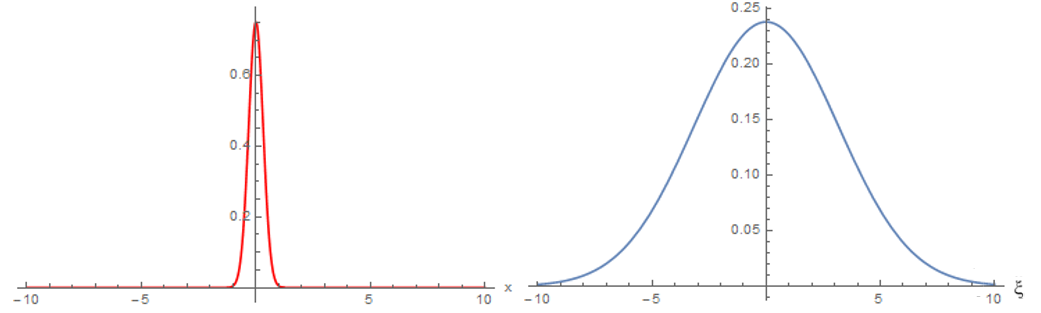
\includegraphics[width=\linewidth]{SsmQdfAqUr-heisen.png}
\end{frame}


\begin{frame}{Princípio da Incerteza de Heisenberg (1927)}
\begin{itemize}Assumimos:
    
    \item $\psi$ representa a "state function";
    \item $\psi \in \mathcal{S}(\mathbb{R})$ e $\int_\mathbb{R}{|\psi(x)|^2dx}=1$;
    \item a probabilidade da partícula estar no intervalo $(a,b)$ é dada por $\int_a^b{|\psi(x)|^2dx}$;
    \item a probabilidade do momento da partícula pertencer ao intervalo $(a,b)$ é dada por $\int_a^b{|\hat{\psi}(\xi)|^2d\xi}$
\end{itemize}



    $$ \Big( \int_{-\infty}^{\infty}{x^2 |\psi(x)|^2dx} \Big)  \Big( \int_{-\infty}^{\infty}{\xi^2 |\hat{\psi}(\xi)|^2d\xi} \Big) \geq \frac{1}{16\pi^2}$$
    $$(\text{incerteza na posição)} \times \text{(incerteza no momento)} \geq \frac{1}{16\pi^2}$$
\end{frame}

\begin{frame}{Princípio da Incerteza de Hardy (1933)}
    \begin{block}{Teorema (Hardy)}
        Seja $f: \mathbb{R} \rightarrow\mathbb{C}$ tal que
        $f(x)=O(e^{-\pi ax^2})$ \text{e} $\hat{f}(\xi)=O(e^{-\pi b \xi^2})$, com $a,b > 0 $, então:
        \begin{itemize}
            \item se $ab=1$, então $f$ é um múltiplo escalar de $e^{- \pi a x^2}$
            \item se $ab >1$, então $f$ é a função identicamente nula.
        \end{itemize}
    \end{block}
\end{frame}

\begin{frame}{Próximos Passos}
\textcolor{gray}{Séries de Fourier}\\
\textcolor{gray}{Transformada de Fourier em $\mathbb{R}$};\\
Transformada de Fourier em $\mathbb{R}^d$;\\
Expressão dos princípios da incerteza em diferentes áreas.

    
\end{frame}

\end{document}
